\documentclass[a5paper, 9pt]{extarticle}
\usepackage[utf8]{inputenc}    % Encodage des caractères
\usepackage[T1]{fontenc}       % Encodage de la police
\usepackage[french]{babel}     % Langue du document
\usepackage{graphicx}          % Pour inclure des images
\usepackage[a5paper, left=1cm, right=1cm, top=1cm, bottom=1cm]{geometry}
\usepackage{marvosym}
\usepackage{enumitem}
\usepackage{titlesec}


%% \newcommand{\linednote}[1]{\par\noindent\textbf{#1}\quad}

%% \newcommand{\linednote}[2]{
%%   \noindent
%%   \begin{minipage}[t]{0.9cm}
%%     \small
%%     \textbf{#1}
%%   \end{minipage}%
%%   %% \hspace{0.1cm}
%%   \begin{minipage}[t]{\dimexpr\linewidth-0.9cm\relax}
%%     \normalsize
%%     #2
%%   \end{minipage}
%%   \vspace*{1mm}
%% }

\newcommand{\linednote}[2]{
  \noindent
  \parbox[t]{0.9cm}{\small \textbf{#1}}%
  \parbox[t]{\dimexpr\linewidth-0.9cm}{\normalsize #2 \vspace{0.4em}}
  \newline
}

\titlespacing{\subsection}{0pt}{*1}{*0.5}  % (indentation, espace avant, espace après)

\title{Paroisse Saint Martin}
\date{\today}

\pagestyle{empty}


\begin{document}

\noindent
\begin{minipage}[t]{0.4\textwidth}
    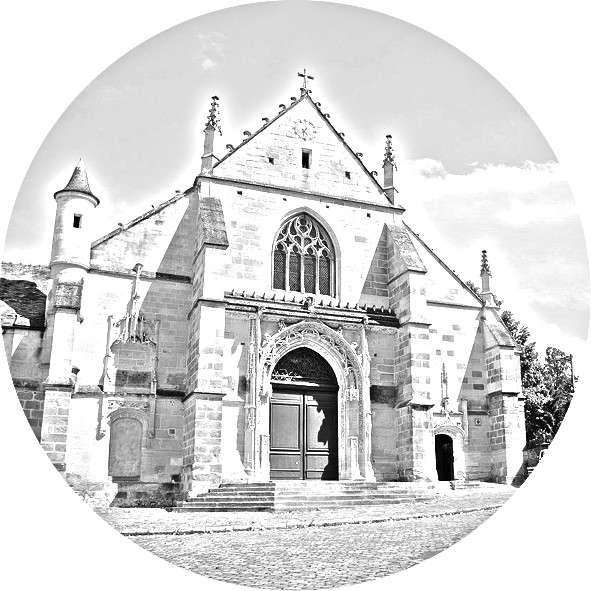
\includegraphics[width=\linewidth]{images/eglise_rond.jpg} % Remplacez par le chemin de votre image
\end{minipage}%
\begin{minipage}[t]{0.55\textwidth}
    \vspace{-3cm} % Ajustez cette valeur pour aligner verticalement avec l'image
    \centering
    % Titre
    {\Huge \bfseries Paroisse Saint Martin \par}

    \vspace{0.3cm} % Espace entre le titre et le sous-titre

    % Sous-titre
    {\Huge \itshape de Longjumeau \par}
\end{minipage}

%% \vspace{1cm}

\subsection*{Un peu d'histoire}

Longjumeau doit probablement ses origines à l'existence d'un gué
permettant à la voie romaine reliant Lutetia (Paris) à Genabum
(Orléans) de franchir l'Yvette.

La découverte d'une vaste nécropole, à l'emplacement de l'hôpital,
datant de l'époque mérovingienne (\textsc{IV}\textsuperscript{e}
siècle) témoigne de cette implantation.

Au \textsc{XII}\textsuperscript{e} siècle la ville s'appelait Nogemel
et faisait partie du domaine de Louis \textsc{VI} le Gros. C'est à
cette époque que Longjumeau devint paroisse.

Pourtant l'église actuelle ne serait que du milieu du
\textsc{XIII}\textsuperscript{e}. (La cathédrale de Paris fut édifiée
à peu près à la même époque).

L'orientation de l'église est est/ouest. Cela pour que le peuple
chrétien puisse célébrer la messe en regardant vers le soleil levant.
Le soleil est souvent utilisé à cette époque pour parler du Christ,
lumière pour l'humanité toute entière. Se tourner vers le soleil
levant en célébrant la messe, c'est se rappeler que, le jour de la
résurrection des morts, tous nous serons appelés à regarder vers le
Seigneur et à resplendir comme Lui.

Une des curiosités de notre église c'est la «lanterne des morts» qui
se trouve sur la façade. Anciennement on mettait de ces lanternes dans
les cimetières et elles étaient éclairées certains jours de l'année
pour rappeler à tout le peuple qu'il fallait prier pour les morts.
Notre lanterne est curieuse car c'est une des seules (la seule ?) qui
existe en région parisienne et aussi parce qu'elle a été érigée sur
l'église et non pas sur un des murs du cimetière qui entourait
l'église.

Elle a été classée aux monuments historiques le 1\textsuperscript{er}
avril 1910.

\begin{center}
  \includegraphics[width=0.8\textwidth]{images/eglise_interieur_2.jpg}
\end{center}


\newpage

\subsection*{Le Plan}

\begin{center}
  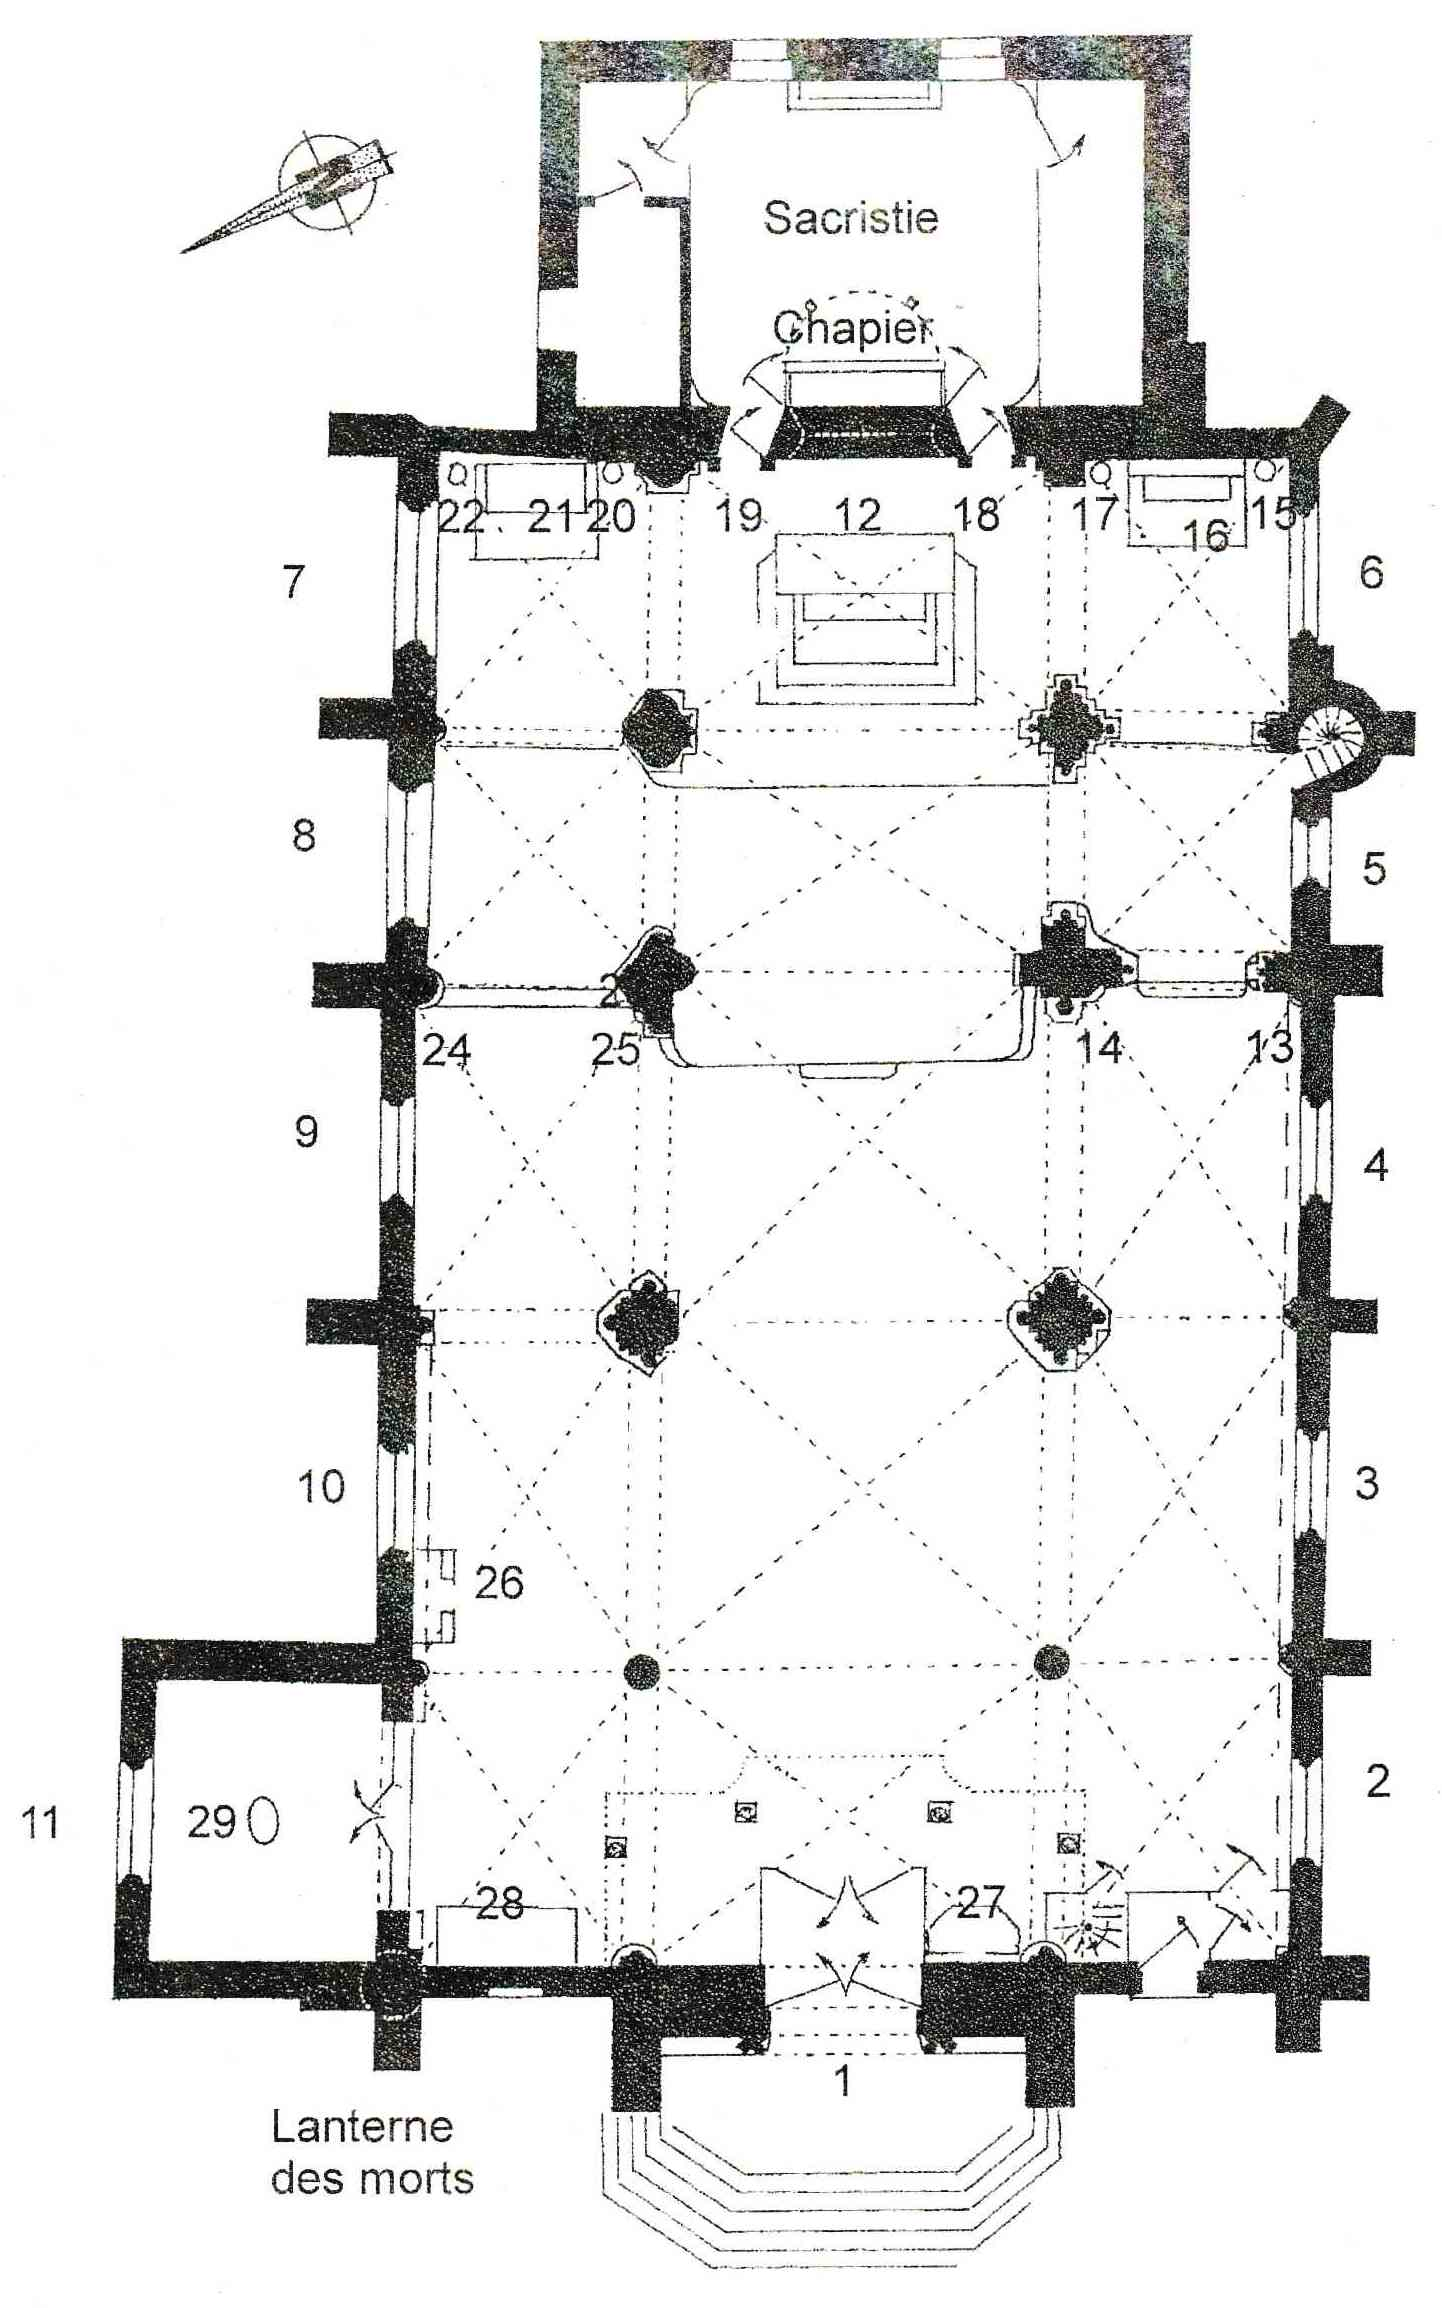
\includegraphics[scale=0.7]{images/plan.jpg}
\end{center}

\subsection*{L'Extérieur}

\linednote{1}{Le \textbf{portail} du \textsc{XV}\textsuperscript{e} siècle, bien que
dépouillé de ses statues lors de la révolution, est d'une grande
beauté. Depuis sa récente restauration il a gagné en dignité et en
prestance.}

\subsection*{Le Chemin de Croix}

Le chemin de croix est réparti tout à long de l'église et des deux
côtés. 14 tableaux rappellent les différents moments de la passion du
Christ. La première station se trouve à la \textbf{chapelle du Sacré
 cœur}, la dernière à la \textbf{chapelle de la Vierge}. Ce sont des
moulages imitant la pierre sculptée datant de 1858.

\subsection*{Les Vitraux}

\linednote{2 3 4}{Vitraux du \textsc{XV}\textsuperscript{e} siècle
restaurés vers le milieu du \textsc{XIX}\textsuperscript{e}.}
\linednote{5}{Vitrail imitant le style du
\textsc{XIII}\textsuperscript{e}. Trois médaillons y représentent, de
bas en haut:
\begin{itemize}[noitemsep,label=\textbullet]
  \item La présentation de \textbf{Marie au Temple}. Ses parents sont
    là, Anne et Joachim.
  \item \textbf{L'Annonciation}. L'ange Gabriel vient annoncer à Marie
    qu'elle va concevoir un fils par l'œuvre de l'Esprit Saint.
  \item \textbf{Le couronnement dans la Gloire de Marie}, mère de
    Dieu, par son Fils, le Christ.
  \item La partie basse de ce vitrail représente \textbf{trois prêtres
    de la paroisse} vers 1866 date d'acquisition de ce vitrail.
\end{itemize}}
\linednote{6}{Vitrail de \textbf{la Sainte Vierge}. Marie, resplendissante, est
en train d'écraser la tête du serpent comme il est dit dans le dernier
livre de la Bible chrétienne.}
\linednote{7}{Dans la chapelle du Sacré cœur, vitrail de 1865,
  représentant \textbf{le repas de Jésus avec les disciples à Emmaüs}.
  Ce dîner, pris le jour même de la Résurrection, est la première
  «messe» célébrée en mémoire du Christ, présidée par Jésus lui-même !}
\linednote{8}{Vitrail de 1865, représentant de gauche à droite:
\begin{itemize}[noitemsep,label=\textbullet]
  \item \textbf{Saint Laurent}, patron d'une maladerie à Longjumeau.
  \item \textbf{Sainte Anne} en train d'enseigner la Parole de Dieu à
    sa fille, Marie.
  \item \textbf{Saint Eloi}, patron d'un prieuré à Longjumeau pendant
    près de 6 siècles.
\end{itemize}}
\linednote{9}{Vitrail de \textbf{l'épiphanie}. Adoration de l'enfant par les
foules et en particulier les mages venus d'orient. Le médaillon du bas
nous dit qu'il a été offert par la municipalité en 1976.}
\linednote{10}{\textbf{Remise de la couronne d'épines à Saint Louis} par André
de Longjumeau en 1239. dans la partie gauche on remarque le toit de la
Sainte Chapelle à Paris, et dans la partie droite le clocher de
Longjumeau tel qu'il était à l'époque.}
\linednote{11}{Vitrail du \textbf{baptême de Jésus par Jean le Baptiste}.
À gauche on distingue trois personnes \dots certainement les deux
premiers disciples qui ont suivi Jésus au lendemain de son baptême et
une femme, peut-être Marie. Il a été acquis grâce aux dons de tous les
chrétiens baptisés à Longjumeau et en particulier de sept prêtres nés
dans la ville. En bas à gauche sont représentés trois de ces sept
prêtres. La partie droite représentant les quatre autres prêtres a été
cassée lors des bombardements de 1944. Les deux anges en haut à droite
et à gauche, sont les petits enfants de deux bienfaiteurs de la
paroisse baptisés à Longjumeau en 1861 et 1863. Ce vitrail daterait de
1865.}
\linednote{12}{Vitrail de \textbf{Saint Martin}, notre Saint Patron,
  partageant son manteau avec un pauvre. Il a été payé par les quêtes
  et les dons des paroissiens en 1877.}

\subsection*{Les Saints}

\linednote{13}{\textbf{Sainte Jeanne d'Arc} en tenue de combat avec l'étendard.
(1412 \Cross 1431) Elle est patronne secondaire de la France.}
\linednote{14}{\textbf{Sainte Thérèse de Lisieux}. Portant l'habit des
carmélites, elle tient en main un crucifix et des roses. Juste avant
de mourir elle avait déclaré qu'elle allait passer son ciel à faire du
bien sur la terre et qu'une pluie de pétales de roses en serait le
signe. Elle est patronne des missions et patronne secondaire de la
France.}
\linednote{15}{\textbf{Notre Dame de Lourdes} telle que l'a décrite Bernadette
  après les apparations de 1858.}
\linednote{16}{Statue en plâtre identique à celle qui se trouve à
  Paris à \textbf{Notre Dame des \mbox{Victoires}}. Elle aurait été
  installée vers la fin du \textsc{XIX}\textsuperscript{e} siècle.}
\linednote{17}{\textbf{Notre Dame de Fatima} telle que l'ont décrite les petits
voyants de 1917 à la «Cova da Iria» au Portugal.}
\linednote{18}{Bien que nous parlions toujours de la «paroisse Saint
Martin», il semblerait que nous avons une co-patronne. Cette Statue de
\textbf{Sainte Anne} placée dans le chœur de l'église et en pendant à Saint
Martin nous l'attesterait.}
\linednote{19}{\textbf{Saint Martin} en habits d'évêque de Tours. Comme la
statue de Sainte Anne, cette statue est en pierre. Ces deux statues
ont été acquises en 1882.}
\linednote{20}{\textbf{Saint Jean l'évangéliste}. À ne pas confondre avec Saint
Jean le Baptiste. Il tient en mains un rouleau de la Parole de Dieu.}
\linednote{21}{\textbf{Sacré cœur de Jésus}. Au dessous devrait se trouver le
tabernacle de la paroisse. Il est actuellement sur le maître autel.}
\linednote{22}{\textbf{Saint Joseph}, l'époux de Marie et père nourricier de
Jésus. Il tient une équette de charpentier et une fleur de lys symbole
de la virginité.}
\linednote{23}{\textbf{Saint Antoine de Padoue}. On l'invoque souvent pour les
causes désespérées.}
\linednote{24}{\textbf{Saint Michel}. Son nom signifie en hébreu «qui est comme
Dieu» (MI KA EL). Il est considéré dans la Bible comme le chef des
armées célestes, c'est pourquoi on le représente presque toujours en
train de combattre le mal représenté souvent par un dragon.}
\linednote{25}{\textbf{Sainte Anne} en train de donner un cours à
  \textbf{Marie}. On représente presque toujours Sainte Anne en train
  d'éduquer sa fille.}

\subsection*{Le Mobilier}

\linednote{26}{\textbf{Confessionnal} de 1859.}
\linednote{27}{\textbf{Confessionnal} de 1755.}
\linednote{28}{\textbf{Banc d'œuvre} datant du \textsc{XVIII}\textsuperscript{e} siècle.}
\linednote{29}{\textbf{La cuve baptismale} a été acquise en 1860. Elle est en marbre rose veiné.}

\subsection*{Le Maître Autel}

\textbf{Le maître autel} est de la fin du \textsc{XIX}\textsuperscript{e}
siècle. Il est en pierre de Caen. Il fut consacré le 30 septembre
1877. Il est de style \textsc{XIII}\textsuperscript{e} et s'harmonise
assez bien avec l'ensemble du bâtiment. De Chaque côté du tabernacle
qui est au centre, trois compartiment sont peints avec des saints bien
connus de notre région. De gauche à droite:
\begin{itemize}[noitemsep,label=\textbullet]
  \item \textbf{Saint Vincent de Paul} en habits de prêtre. (1581 \Cross 1660)
  \item \textbf{Saint Louis}, roi de France. (1214 \Cross 1270)
  \item \textbf{Saint Denis}, premier évêque de Paris. (? \Cross 272)
  \item \textbf{Saint Eloi}, évêque de Noyon. (588 \Cross 660)
  \item \textbf{Saint Laurent}, avec la palme signifiant qu'il est mort en martyr. (215 \Cross 258)
  \item \textbf{Sainte Geneviève}, vierge, née à Nanterre et morte à Paris. (423 \Cross 512)
\end{itemize}

\vspace*{\fill}

Beaucoup de ces données ont été trouvées dans une excellente plaquette
de l'association Renaissance et Culture de Longjumeau et ses environs;
d'autres trouvées sur Wikipedia ou dans les archives paroissiales.

\vspace*{\fill}

\begin{flushbottom}
  \begin{center}
    \scriptsize Version : \today
  \end{center}
\end{flushbottom}

\end{document}
